\subsection{System Architecture}

The system architecture of aBridgeAI is designed as a modern, decoupled structure that clearly delineates the \textbf{system boundary}---separating internal processing components from external actors and third-party service providers. This separation ensures that the system can evolve independently of its environment while maintaining well-defined interfaces for all external interactions.

\subsubsection{Actors and External Environment}
Before describing the internal architecture, it is essential to identify all actors and external services that exist \textit{outside} the system boundary and interact with it through defined interfaces.

\paragraph{System Actors (Users)}
Five distinct user roles interact with the aBridgeAI system, each with specific access privileges and operational responsibilities:

\begin{enumerate}
    \item \textbf{Student:} The primary end-user who accesses course materials, completes SR review sessions, takes assessments, and participates in AI-driven voice interviews. Students interact with the system exclusively through web browsers or mobile devices.
    \item \textbf{Instructor:} The content creator and pedagogical authority. Instructors design courses, define learning outcomes, configure assessment parameters (e.g., SR thresholds, interview difficulty levels), and review aggregated student performance analytics including knowledge retention reports.
    \item \textbf{Education Manager:} The organizational administrator responsible for provisioning the learning environment. This role creates and manages user accounts, establishes course structures, assigns instructors to courses, enrolls students, and oversees institutional-level analytics and reporting.
    \item \textbf{Faculty Dean:} The academic authority over one faculty, holding the full authority of an Education Manager within that scope and, in addition, the governance decisions that belong to a faculty rather than to the organisation --- authoring learning programmes and adjudicating student requests to change or drop a career pathway.
    \item \textbf{IT Administrator:} The technical operations role responsible for system health monitoring, infrastructure maintenance, deployment management, and troubleshooting.
\end{enumerate}

\paragraph{External Service Providers}
The system integrates with several third-party services that reside outside the system boundary:

\begin{itemize}
    \item \textbf{Identity Provider (Google OAuth 2.0):} Provides delegated authentication via the user's Google account. The platform issues its own session JWTs and persists second-factor enrolment (TOTP) in its internal database.
    \item \textbf{LLM and Embedding Provider:} Supplies inference and embedding capabilities consumed by the AI layer. The platform targets the OpenAI-compatible chat-completions and embeddings interface rather than one vendor's SDK, so the provider is a configured base URL and model identifier per role; the models evaluated in Chapter~\ref{sec:evaluation} are open-weight models served through that interface.
    \item \textbf{Speech Services (Deepgram):} Provides voice transcription and synthesis during real-time interview sessions --- streaming speech-to-text for English and Vietnamese, and text-to-speech for English narration --- integrated through the LiveKit agent pipeline.
\end{itemize}

\subsubsection{Internal System Components}
The internal architecture is segregated into specialized layers within the system boundary:

\begin{itemize}
    \item \textbf{Frontend Application (Vite + React + TanStack Query):} Serves as the primary client interface, providing a responsive SPA environment. All routes require authentication; there is no public-facing content, making SSR unnecessary. TanStack Query manages server-state with fine-grained cache invalidation and background refetching.

    \item \textbf{Reverse Proxy \& API Gateway (Nginx):} Acts as the single ingress point into the system boundary. Handles HTTPS/TLS termination, load balancing, and routes API requests and WebSocket upgrades to the internal services. Rate limiting is additionally enforced in the backend, so a request reaching the API directly is still bounded.

    \item \textbf{Backend Core \& Orchestration (FastAPI):} The central processing hub. Built on Python for native AI/ML ecosystem access, it handles business logic, RESTful API endpoints, async I/O via \texttt{asyncio}, SR scheduling (SM-2), knowledge retention computation, and AI pipeline orchestration.

    \item \textbf{Real-Time Voice Agent (LiveKit):} Manages ultra-low latency WebRTC (UDP) audio streams. Provides built-in VAD, speaker interruption handling, and conversational turn-taking for AI-driven interviews. The LiveKit Agents SDK coordinates STT, LLM inference, and TTS within a single real-time session.

    \item \textbf{AI Layer (first-party):} A purpose-built package rather than a general orchestration framework, comprising a model gateway that routes each call by its role and records tokens, latency and cost; an extraction, preprocessing and chunking chain; a retrieval stack implementing dense vector search, sparse full-text search, rank fusion, diversification and access filtering as separate modules; and versioned prompt templates. The decision not to adopt a chain-composition framework keeps the retrieval steps individually testable and the per-call audit record exact, which the cost telemetry and the generation-quality evaluation both depend on.

    \item \textbf{Primary Data Store (PostgreSQL + pgvector):} Unified relational and vector database with full ACID compliance. Stores structured data and high-dimensional vector embeddings via \texttt{pgvector}, enabling combined SQL + vector similarity queries within single transactions.

    \item \textbf{Graph Database (Neo4j):} Stores the Course Knowledge Graph. Enables native multi-hop traversal for concept relationship queries, prerequisite chain resolution, and knowledge gap analysis via Cypher queries and APOC algorithms.

    \item \textbf{Cache \& Task Queue (Redis):} In-memory store serving four roles: session caching on the authenticated hot path, API rate limiting (sorted sets), background job scheduling via the \texttt{arq} worker framework for SR card scans and generation jobs, and ownership of a live quiz attempt under compare-and-set scripts. The first three degrade to the database on failure; the last deliberately fails closed.

    \item \textbf{Object Storage (Garage S3):} Self-hosted S3-compatible object store for course material files, uploaded documents, and media assets. Eliminates vendor lock-in while maintaining AWS S3 API compatibility.
\end{itemize}

\subsubsection{System Boundary Diagram}

Figure~\ref{fig:system-diagram} illustrates the high-level system architecture, delineating the system boundary that separates internal components from external actors and third-party service providers.

\begin{figure}[H]
\centering
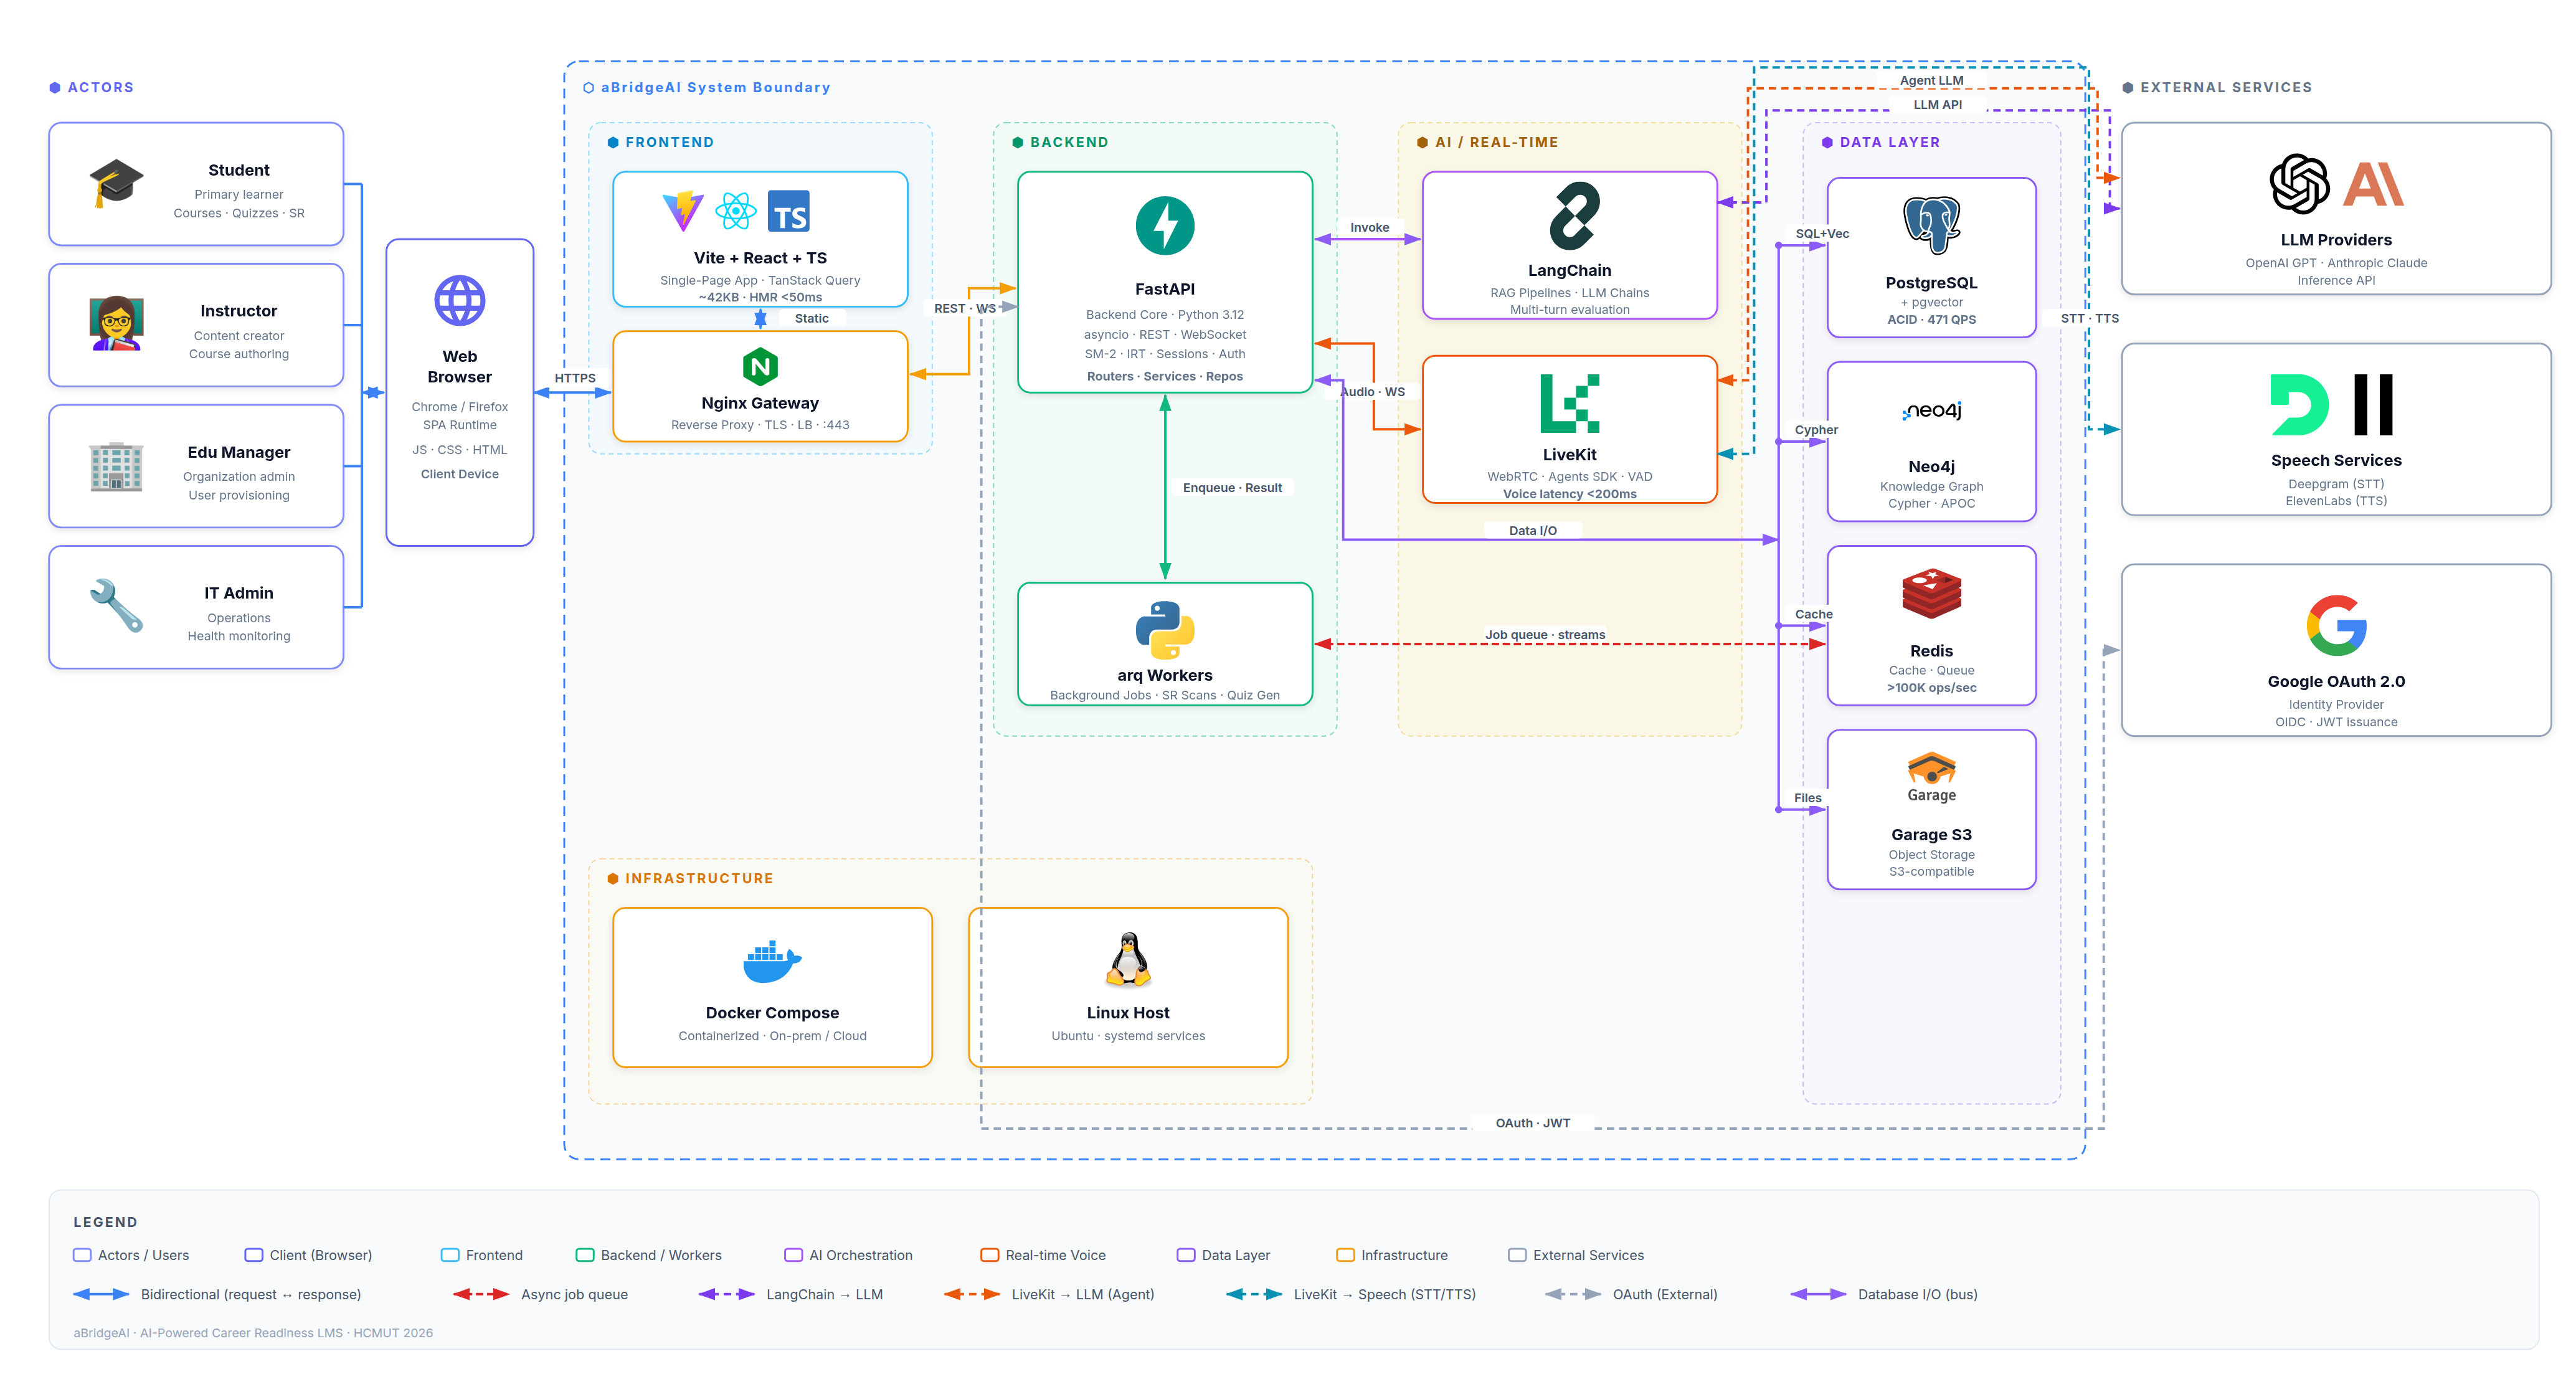
\includegraphics[width=\textwidth]{graphics/system/system_architecture_diagram.png}
\caption{aBridgeAI System Architecture Diagram}
\label{fig:system-diagram}
\end{figure}

\subsubsection{Deployment Architecture}
The aBridgeAI system is deployed as a set of long-running processes behind \textbf{Nginx}, which serves as the reverse proxy and API gateway and terminates TLS. The presentation layer is a \textbf{Vite + React} SPA served as static assets; the application itself runs as three supervised processes rather than one, and the separation is deliberate. A \textbf{FastAPI} service under Uvicorn serves the API; an \texttt{arq} \textbf{worker} consumes the job queue, so ingestion and generation cannot block a request or be lost to a web-process restart; and a \textbf{LiveKit interview agent} runs independently, because a real-time voice session has a lifetime measured in minutes and must survive an API deployment.

The backing services --- \textbf{PostgreSQL with pgvector} for relational and vector data, \textbf{Neo4j} for the Course Knowledge Graph, \textbf{Redis} for caching, rate limiting, queueing and attempt ownership, and \textbf{Garage} as a self-hosted S3-compatible object store --- are containerised. Clients transfer material to and from the object store through presigned URLs issued by the API rather than streaming bytes through it, so upload size is bounded by storage policy rather than by request timeouts.

The AI layer is first-party code calling an OpenAI-compatible provider over HTTP, with no chain-orchestration framework between them. \textbf{LiveKit} handles real-time WebRTC voice sessions for interviews, coordinating \textbf{Deepgram} speech-to-text and text-to-speech within a single session.

This architecture separates concerns across routing, application logic, storage, AI processing, and real-time delivery, making the system scalable, maintainable, and deployable on both cloud and on-premise infrastructure.
